\documentclass[a4paper]{article}
\usepackage{float}
\usepackage[english]{babel}
\usepackage[utf8]{inputenc}
\usepackage{amsmath}
\usepackage{mathtools}
\usepackage{amsfonts}
\usepackage{caption}
\usepackage{subcaption}
\usepackage{graphicx}
\usepackage[colorinlistoftodos]{todonotes}
\usepackage{tcolorbox}
\usepackage{tikz}
\usetikzlibrary{bayesnet}
\DeclareMathOperator{\tr}{tr}
\DeclareMathOperator{\vect}{vec}
\DeclareMathOperator{\etr}{etr}
\DeclareMathOperator{\E}{E}

\title{Assignment 1}

\author{Marcus Lindström}

\date{\today}

\begin{document}
\maketitle

\section{The Prior}
\subsection{Theory}

\noindent\textbf{Q1} 

\noindent\makebox[\linewidth]{\rule{\textwidth}{0.4pt}}

\hfill

\noindent The Central Limit Theorem states that the normalized sum of independent random variables are approximately normally distributed. The likelihood depends only on the uncertainty in $x_i$, and it's rather safe to assume that observation errors can be thought of as sums of many different error sources that are independent of each-other, that together with the fact that Gaussian's are rather mathematically convenient to work with makes it a sensible choice. Using a spherical covariance means that dimensions of $\mathbf{t_i}$ are independent and have equal uncertainty.    \\

\noindent \textbf{Q2}

\noindent\makebox[\linewidth]{\rule{\textwidth}{0.4pt}}

\begin{equation*}
p(\mathbf{T}\vert f,\mathbf{X})=p(\mathbf{t}_N\vert f, \mathbf{X})\prod_{i=1}^{N-1}p(\mathbf{t}_i\vert \mathbf{t}_{i+1},...,\mathbf{t}_{N-1},\mathbf{t}_{N},f, \mathbf{X})
\end{equation*}

\hfill

\noindent \textbf{Q3}

\noindent\makebox[\linewidth]{\rule{\textwidth}{0.4pt}}

\begin{equation*}
p(\mathbf{T}\vert \mathbf{X},\mathbf{W}) = \prod_{i=1}^{N}\mathcal{N}(\mathbf{t}_i\vert \mathbf{W}\mathbf{x}_i,\sigma^2\mathbf{I})
\end{equation*}

\noindent \textbf{Q4}

\noindent\makebox[\linewidth]{\rule{\textwidth}{0.4pt}}


\begin{figure*}[t!]
	\centering
	\begin{subfigure}[t]{0.5\textwidth}
		\centering
		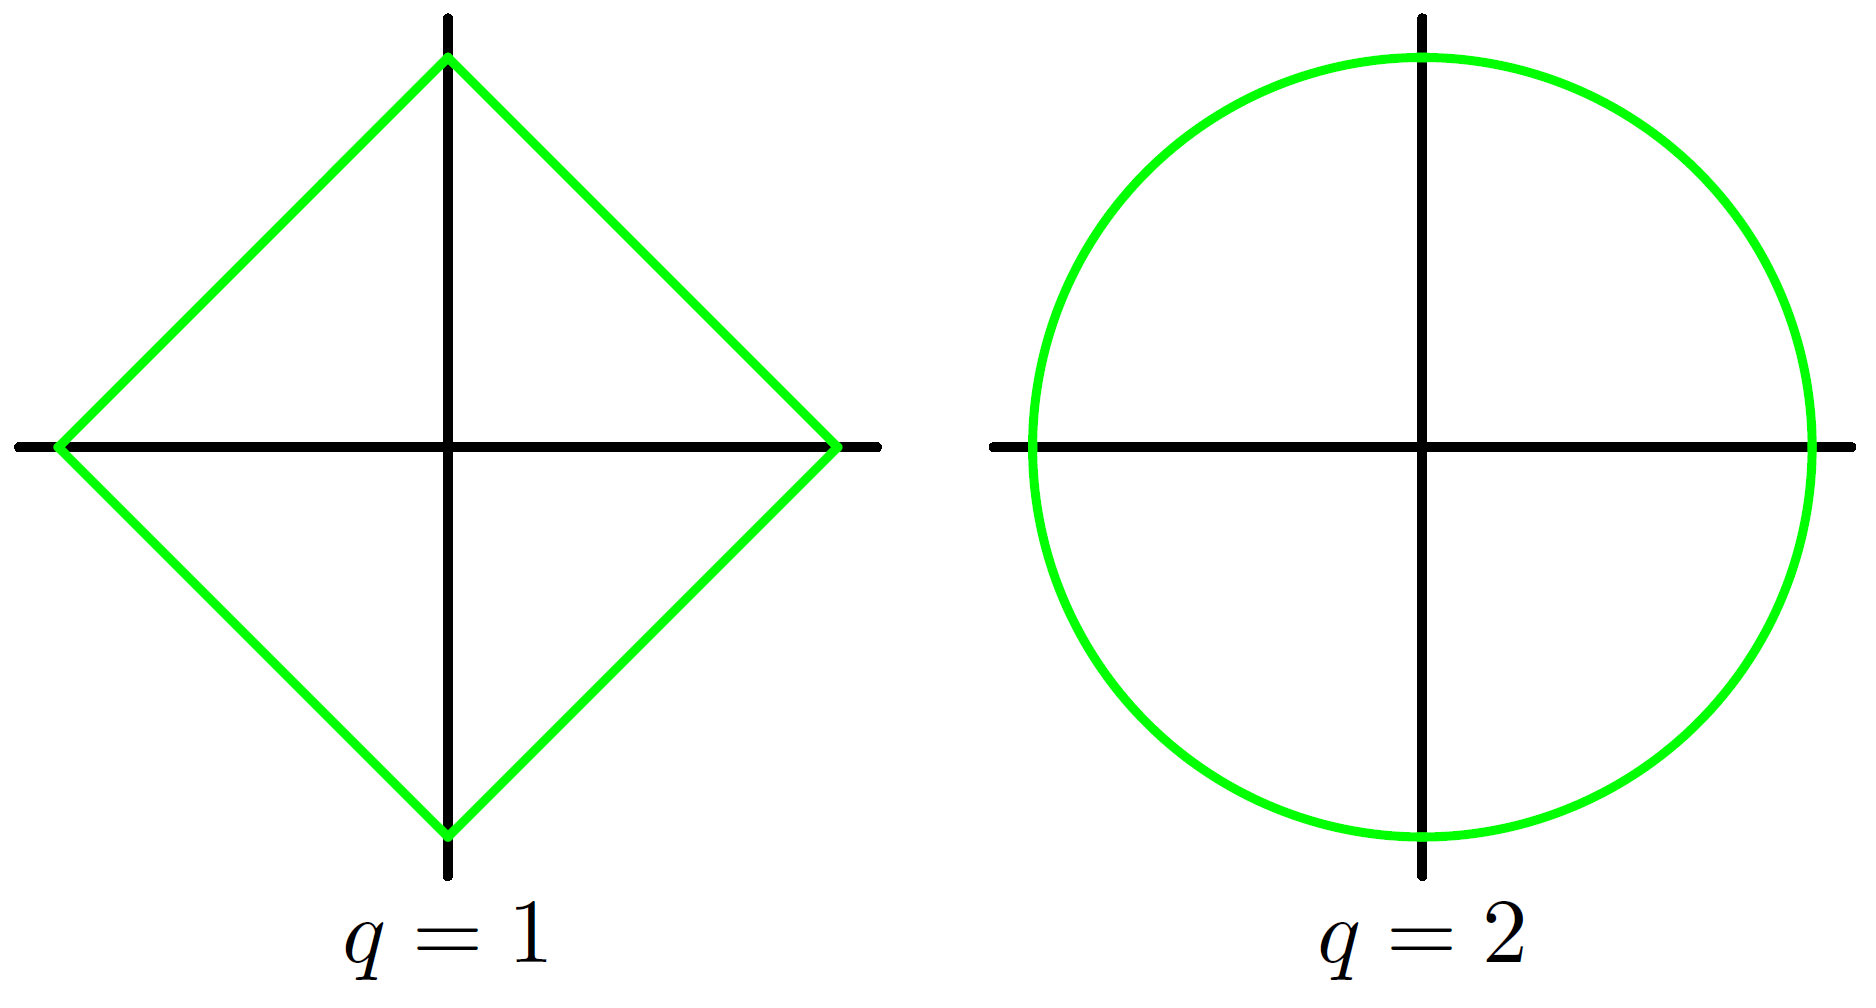
\includegraphics[height=1.4in]{L2.png}
		\caption{$L1$ \& $L2$ priors encoding comparison, picture taken from Bishop, page 145.}
	\end{subfigure}%
	~ 
	\begin{subfigure}[t]{0.5\textwidth}
		\centering
		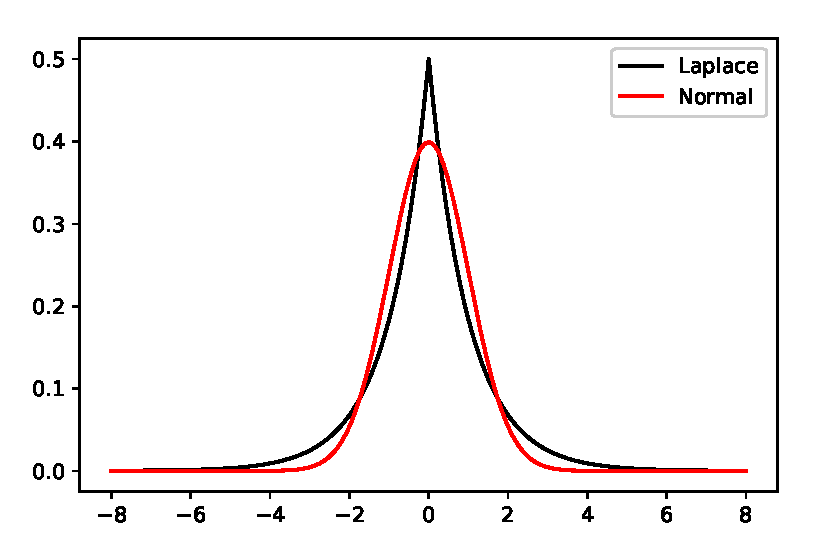
\includegraphics[height=1.4in]{Place.eps}
		\caption{One dimensional illustration.}
	\end{subfigure}
\end{figure*}

\noindent A generalized penalization term $E_p$ i.e. the negative log-prior has the following form where $\lambda$ is a constant:

\begin{equation*}
E_p=\lambda\sum_{i=1}^{M}\vert w_i\vert^{q}
\end{equation*}

\noindent Where $q=1$ and $q=2$ result in $L_1$ and $L_2$ respectively. How we encode the prior expresses our belief in the model parameters, and we see in the picture below that using a $L1$ prior, you are more prone to end up with many zero-valued parameters, but due to the long tail of the distribution, some parameters might also be large-sized. $L2$ is more smooth around zero, so non-zero values have greater probability and are less likely to end up at zero.

\hfill

\noindent\textbf{Q5} 

\noindent\makebox[\linewidth]{\rule{\textwidth}{0.4pt}}

\hfill

\noindent Using the notation, $\etr(\cdot)\equiv\exp(\tr(\cdot))$, we can rewrite our likelihood and prior distributions with help of vectorization using the identity $\vect(\mathbf{A})^T\vect(\mathbf{B})=\tr(\mathbf{A}^T\mathbf{B})$:

\begin{align*}
\begin{split}
p(\mathbf{T}\vert \mathbf{X},\mathbf{W})&= \prod_{i=1}^{N}\mathcal{N}(\mathbf{t}_i\vert \mathbf{W}\mathbf{x}_i,\sigma^2\mathbf{I}) \propto \exp \bigg(-\frac{1}{2\sigma^2}\sum_{i=1}^{N}(\mathbf{t}_i-\mathbf{W}\mathbf{x}_i)^T(\mathbf{t}_i-\mathbf{W}\mathbf{x}_i)\bigg)\\ & = \exp\bigg(-\frac{1}{2\sigma^2}\vect(\mathbf{T-WX})^T\vect(\mathbf{T-WX})\bigg) \\ & = \etr \bigg(-\frac{1}{2\sigma^2}\big[\mathbf{T}^T\mathbf{T}-2\mathbf{T}^T\mathbf{WX}+\mathbf{X}^T\mathbf{W}^T\mathbf{WX}\big]\bigg),
\end{split}\\
\begin{split}
p(\mathbf{W})&= \mathcal{MN}(\mathbf{W}_0,\mathbf{I},\tau^2\mathbf{I}) \propto \etr\bigg[-\frac{1}{2\tau^2}(\mathbf{W}-\mathbf{W}_0)^T(\mathbf{W}-\mathbf{W}_0)\bigg] \\ & = \etr\bigg[-\frac{1}{2\tau^2}\bigg(\mathbf{W}^T\mathbf{W}-2\mathbf{W}^T\mathbf{W}_0+\mathbf{W}_0^T\mathbf{W}_0\bigg)\bigg].
\end{split}\\
\end{align*}

\noindent The posterior according to Baye's is proportional to the product of the likelihood and the prior:

\begin{align*}
\begin{split}
p(\mathbf{W}\vert \mathbf{X},\mathbf{T})\propto\etr\bigg[-\frac{1}{2\sigma^2}\bigg(\mathbf{T}^T\mathbf{T}-2\mathbf{T}^T\mathbf{WX}+\mathbf{X}^T&\mathbf{W}^T\mathbf{WX}\bigg)-\frac{1}{2\tau^2}\bigg(\mathbf{W}^T\mathbf{W}\\&-2\mathbf{W}^T\mathbf{W}_0+\mathbf{W}_0^T\mathbf{W}_0\bigg)\bigg].
\end{split}\\
\end{align*}

\noindent We focus on the terms in the exponent that are either quadratic ($\mathbf{E}_q$) or linear ($\mathbf{E}_l$) in $\mathbf{W}$ and drop the other terms, note that since we are taking the trace of these matrices we can cyclically permute their order and also transpose any term and preserve the equality, doing so and rearranging a bit gives the following:

\begin{equation*}
\mathbf{E}_q = \bigg(\frac{1}{\sigma^2}\mathbf{XX}^T+\frac{1}{\tau^2}\mathbf{I}\bigg)\mathbf{W}^T\mathbf{W},\quad \mathbf{E}_l = \mathbf{W}^T\bigg(\frac{1}{\sigma^2}\mathbf{TX}^T+\frac{1}{\tau^2}\mathbf{W}_0\bigg).
\end{equation*}

\noindent Lets formulate the posterior in its general form, since the likelihood and prior are conjugate we know that the posterior is normal:

\begin{align*}
\begin{split}
p(\mathbf{W}\vert \mathbf{X},\mathbf{T})&=p(\mathbf{X\vert M,U,V})\propto\etr\bigg(-\frac{1}{2}\bigg[\mathbf{V}^{-1}\big(\mathbf{W}-\mathbf{M}\big)^T\mathbf{U}^{-1}(\mathbf{W}-\mathbf{M})\bigg]\bigg) \\ &= \etr\bigg(-\frac{1}{2}\bigg[\underbrace{\mathbf{V}^{-1}\mathbf{W}^T\mathbf{U}^{-1}\mathbf{W}}_{\text{quadratic}}-2\underbrace{\mathbf{W}^T\mathbf{U}^{-1}\mathbf{M}\mathbf{V}^{-1}}_{\text{linear}}+\mathbf{V}^{-1}\mathbf{M}^T\mathbf{M}\bigg]\bigg).
\end{split}\\
\end{align*}

\noindent We can now easily compare the quadratic and linear terms and thus conclude the following:

\begin{equation*}
\mathbf{U}=\mathbf{I},\quad \mathbf{V}^{-1}=\bigg(\frac{1}{\sigma^2}\mathbf{XX}^T+\frac{1}{\tau^2}\mathbf{I}\bigg), \quad \mathbf{M}=\bigg(\frac{1}{\sigma^2}\mathbf{TX}^T+\frac{1}{\tau^2}\mathbf{W}_0\bigg)\mathbf{V}.
\end{equation*}

\noindent The constant $Z$ is a normalizing factor, and looking at the mean and covariance tells us a few things: The mean of the prior does not stretch the posterior so the covariance does not depend on it, the posterior mean does however due to the translation. We also see that both the mean and the covariance of the posterior depends on the data and the uncertainty of it. If we compare the mean to the ML-estimate that is given in Bishop p. 142, we see that if we were to remove $\mathbf{W}_0$ and $\frac{1}{\tau^2}\mathbf{I}$, the expressions would be equivalent.

\hfill

\noindent\textbf{Q6}
 
\noindent\makebox[\linewidth]{\rule{\textwidth}{0.4pt}}

\hfill

\noindent We want the prior to reflect our belief in $\mathbf{f}$ given our data. So we model $\mathbf{K_{\theta}}$ so as to give similar pairs of data $\mathbf{x}_i, \mathbf{x}_j$ high correlation for corresponding instantiations $\mathbf{f}_i, \mathbf{f}_j$, and the opposite for points that are not similar. This is rather subjective, but there are many ways to model this similarity and tune it with hyper-parameters $\mathbf{\theta}$ depending on the scenario.

\begin{figure}[H]
	\centering
	\includegraphics[width=0.4\textwidth]{Heatmap.eps}
	\caption{\label{fig:frog} Visualization of the prior covariance matrix in the $\mathcal{GP}$ using an exponential quadratic kernel with length scale set to 1.2.}
\end{figure}

\noindent We see in figure 2 that the covariance matrix of the prior reflects this behavior, correlations near the diagonal are higher, meaning $f_i$ and $f_j$ correlate more if $i\approx j$. It is also, as is much else that's modeled with a normal distribution very handy to work with e.g. to marginalize over. If we inspect the marginal distribution given in Bishop 6.61,

\begin{equation*}
p(\mathbf{t})=\mathcal{N}(\mathbf{t\vert 0}, \mathbf{C}), \quad C_{i,j}=K_{i,j}+\beta^{-1}\delta_{i,j}.
\end{equation*}

\noindent this means that when evaluating how likely our target values are given our data, with this approach - how uncertain we are depends directly on the noise in our data and the uncertainty in our prior.

\hfill

\noindent\textbf{Q7}

\noindent\makebox[\linewidth]{\rule{\textwidth}{0.4pt}}
\hfill

\noindent The joint distribution is given by

 \begin{equation*}
 p(\mathbf{T,X,f,\theta})=p(\mathbf{T\vert f})p(\mathbf{f\vert X,\theta})p(\mathbf{X})p(\theta).
 \end{equation*}

\noindent $\theta$ and $\mathbf{X}$ are assumed independent, we also make the assumption that $\mathbf{T}$ is conditionally independent of $\theta$ and $\mathbf{X}$ given $\mathbf{f}$ which is also illustrated in the following image:

\begin{figure}[H]
	\centering
	\tikz{ %
		\node[obs]                       		(X)   		{$\mathbf{X}$};
		\node[obs,   below = of X]     			(theta)     {$\theta$};
		\node[obs,   right = of theta, yshift=0.8cm]   		(f) 		{$\mathbf{f}$};
		\node[obs,   right = of f]   			(t) 		{$\mathbf{T}$};
		\edge {X} {f};
		\edge {theta} {f};
		\edge {f} {t};

	}
\end{figure}

\noindent\textbf{Q8}

\noindent\makebox[\linewidth]{\rule{\textwidth}{0.4pt}}

 \begin{equation*}
p(\mathbf{T}\vert\mathbf{X,\theta})=\int \underbrace{p(\mathbf{T}\vert\mathbf{f})}_{\text{likelihood}}\underbrace{p(\mathbf{f}\vert \mathbf{X,\theta})}_{\text{prior}}d\mathbf{f}.
\end{equation*}

\noindent We can look at the integral above as a weighted average of all likelihoods with priors as weights, and since both the likelihood and the prior are Gaussian, the marginal distribution is as-well. This means the uncertainty in both the prior as-well as the noise from the data simply add up, meaning it directly filters through to the marginal distribution. We condition on $\theta$ still because it's assumed constant during integration, to be fully Bayesian we'd marginalize it out but that would be too costly computationally-wise. Now instead, it can be used in order to tune the kernel function.

\newpage

\subsection{Practical}

\subsubsection{Linear Regression}

\noindent\textbf{Q9}

\noindent\makebox[\linewidth]{\rule{\textwidth}{0.4pt}}

\begin{figure}[H]
	\centering
	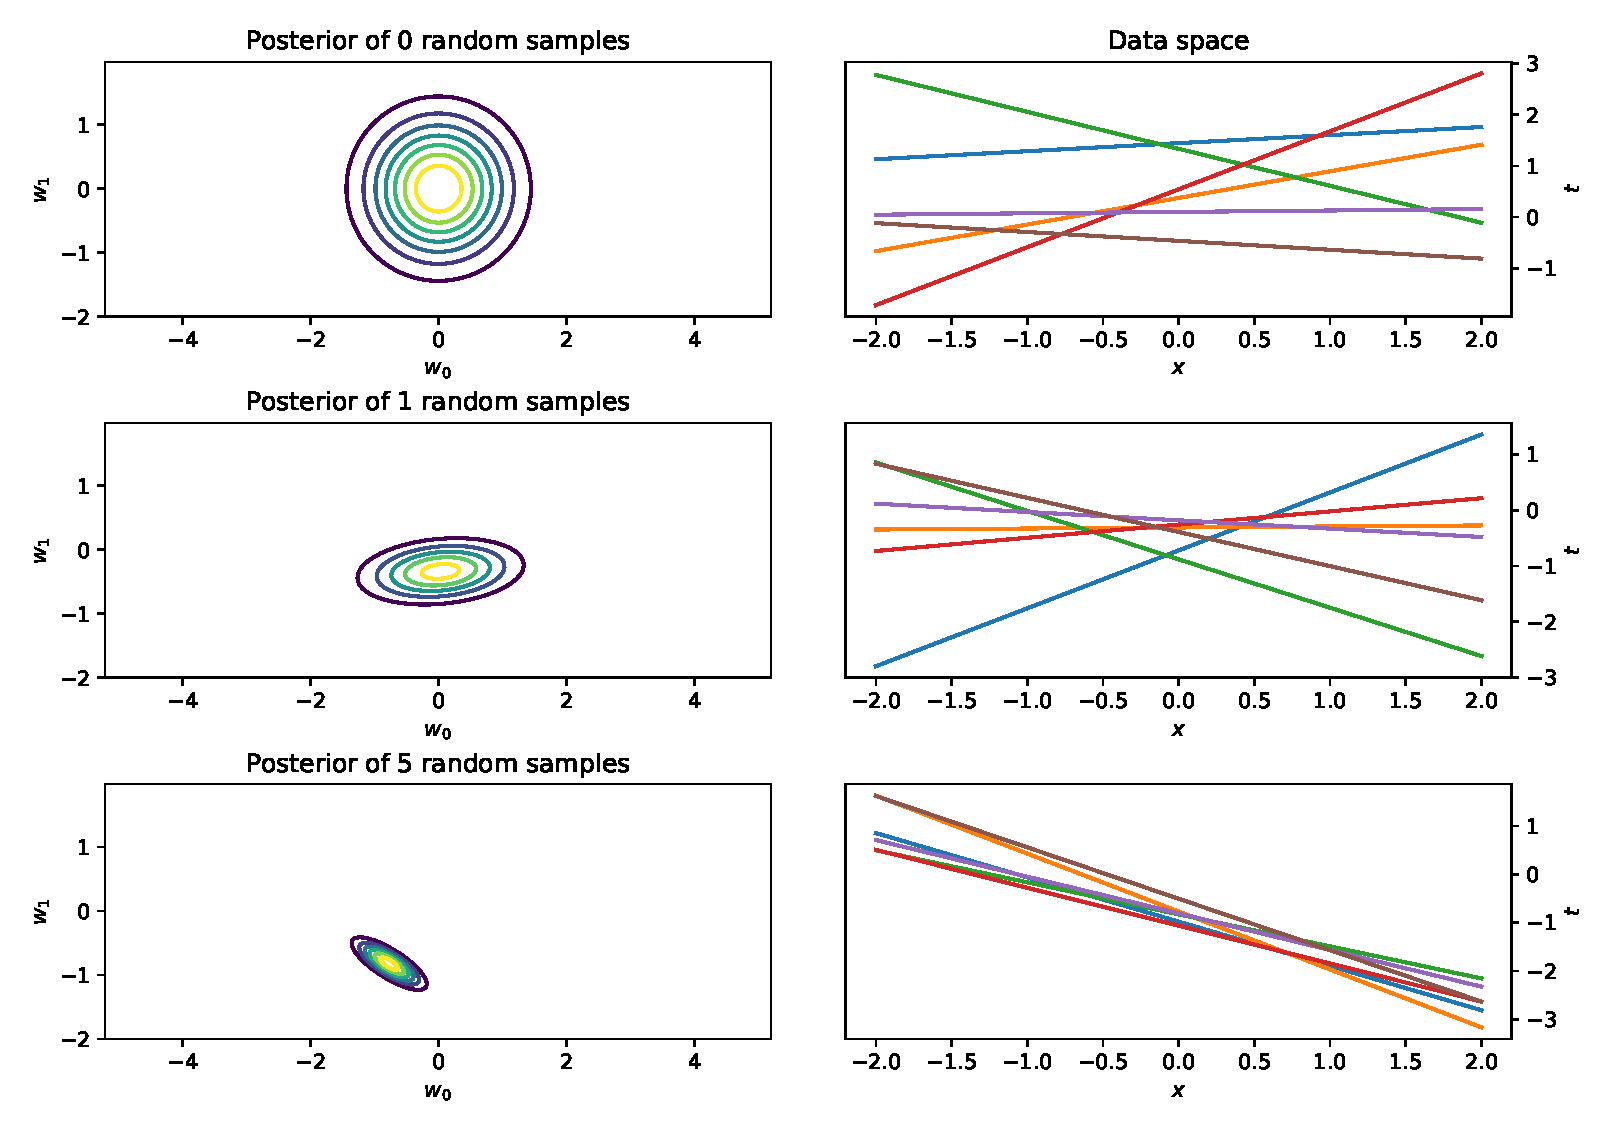
\includegraphics[width=1\textwidth]{foo.eps}
	\caption{\label{fig:frog}Illustration of sequential Bayesian linear regression learning, further explanation is given below.}
\end{figure}

\noindent The prior is given by the top left contour where the precision matrix is set to 2$\mathbf{I}$ and a mean at the origin. Even if it was not asked in the assignment, we chose to sample from it and generate lines based on our prior assumption about the structure of the data. We see in the data space that the prior tends to favor parameters close to zero, which connects to question 4 above. When we add more data, the posteriors get higher precision and we see in the data space that the model is getting closer to the true one. This can be explained from the fact that for each new data point that we add, we use the earlier posterior as our new prior and simply multiply it with the likelihood of our new sample (which can be interpreted as the compatibility of the sample with the given model hypothesis). Thus strengthening our assumption of the model if it continues to generate high likelihood estimates. The test was repeated 3 more times with the addition of trying out different noise levels in the samples, we see in image 4 below that the model predictions get less certain as more noise is added which directly connects to our discussion in question 5.

\begin{figure}[H]
	\centering
	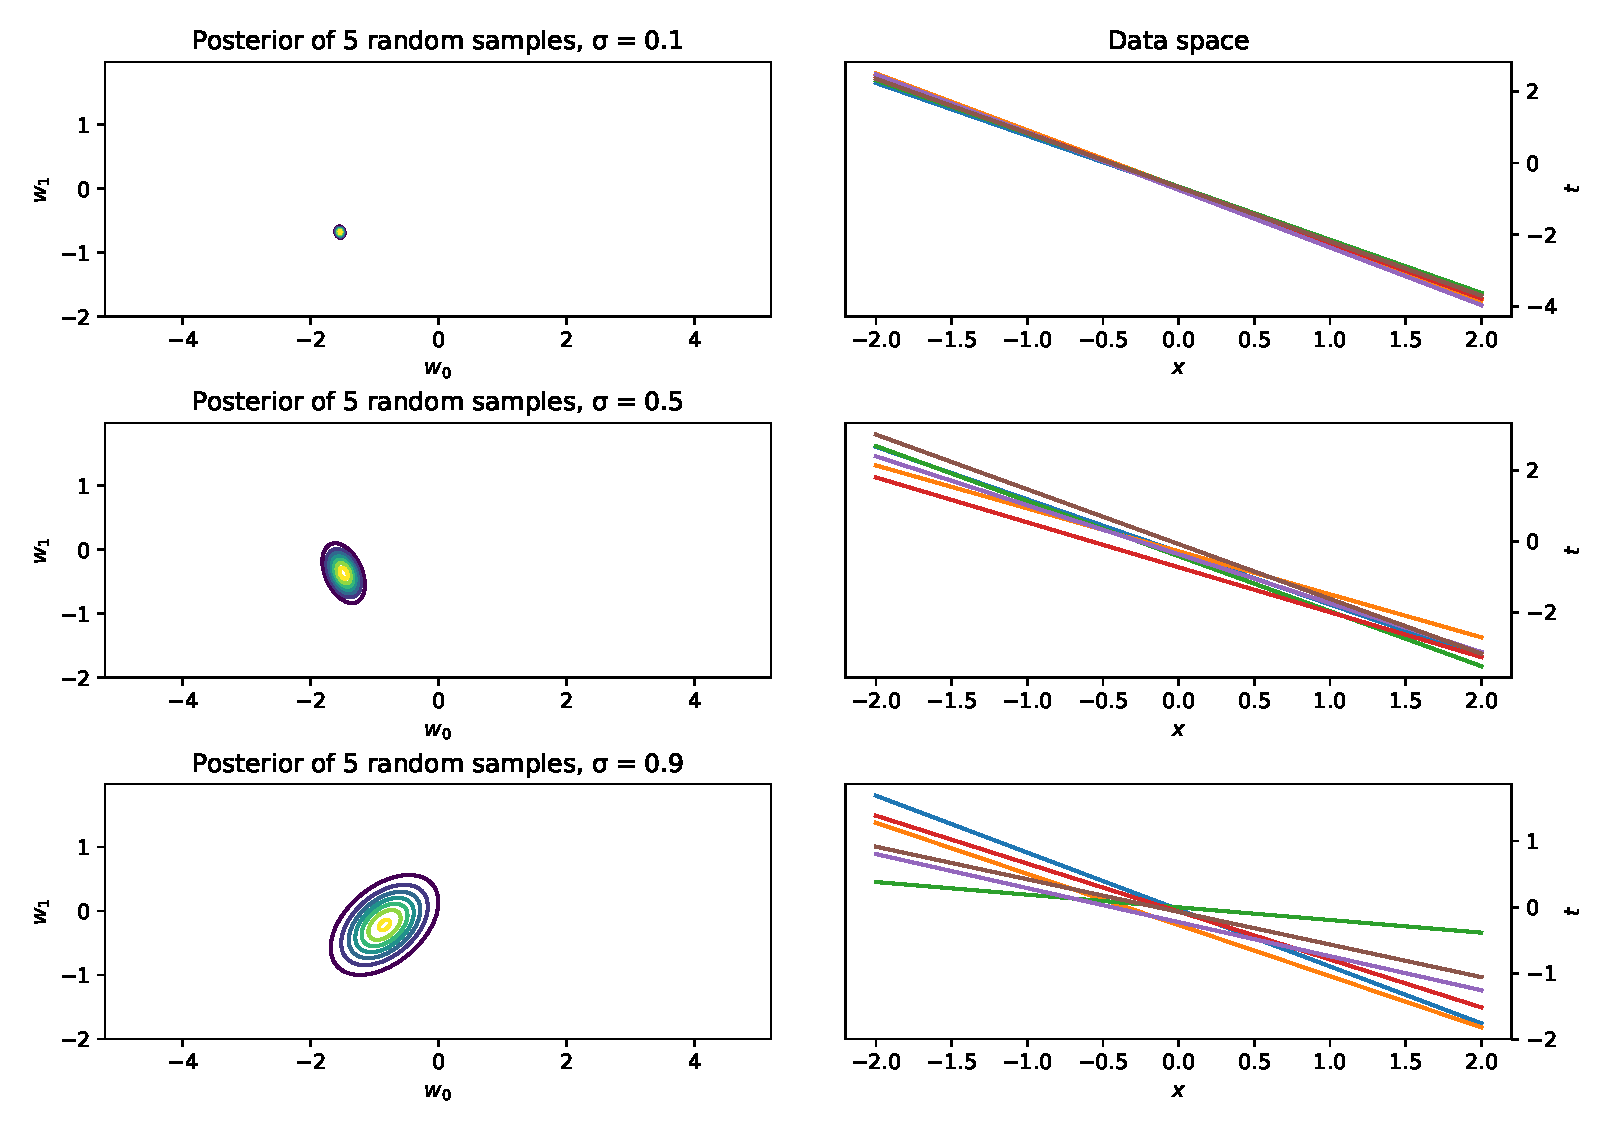
\includegraphics[width=1\textwidth]{foo2.eps}
	\caption{\label{fig:frog} Comparison between using different noise levels for Bayesian linear regression.}
\end{figure}

\newpage

\subsubsection{Non-parametric Regression}

\noindent\textbf{Q10}

\noindent\makebox[\linewidth]{\rule{\textwidth}{0.4pt}}

\begin{figure}[H]
	\centering
	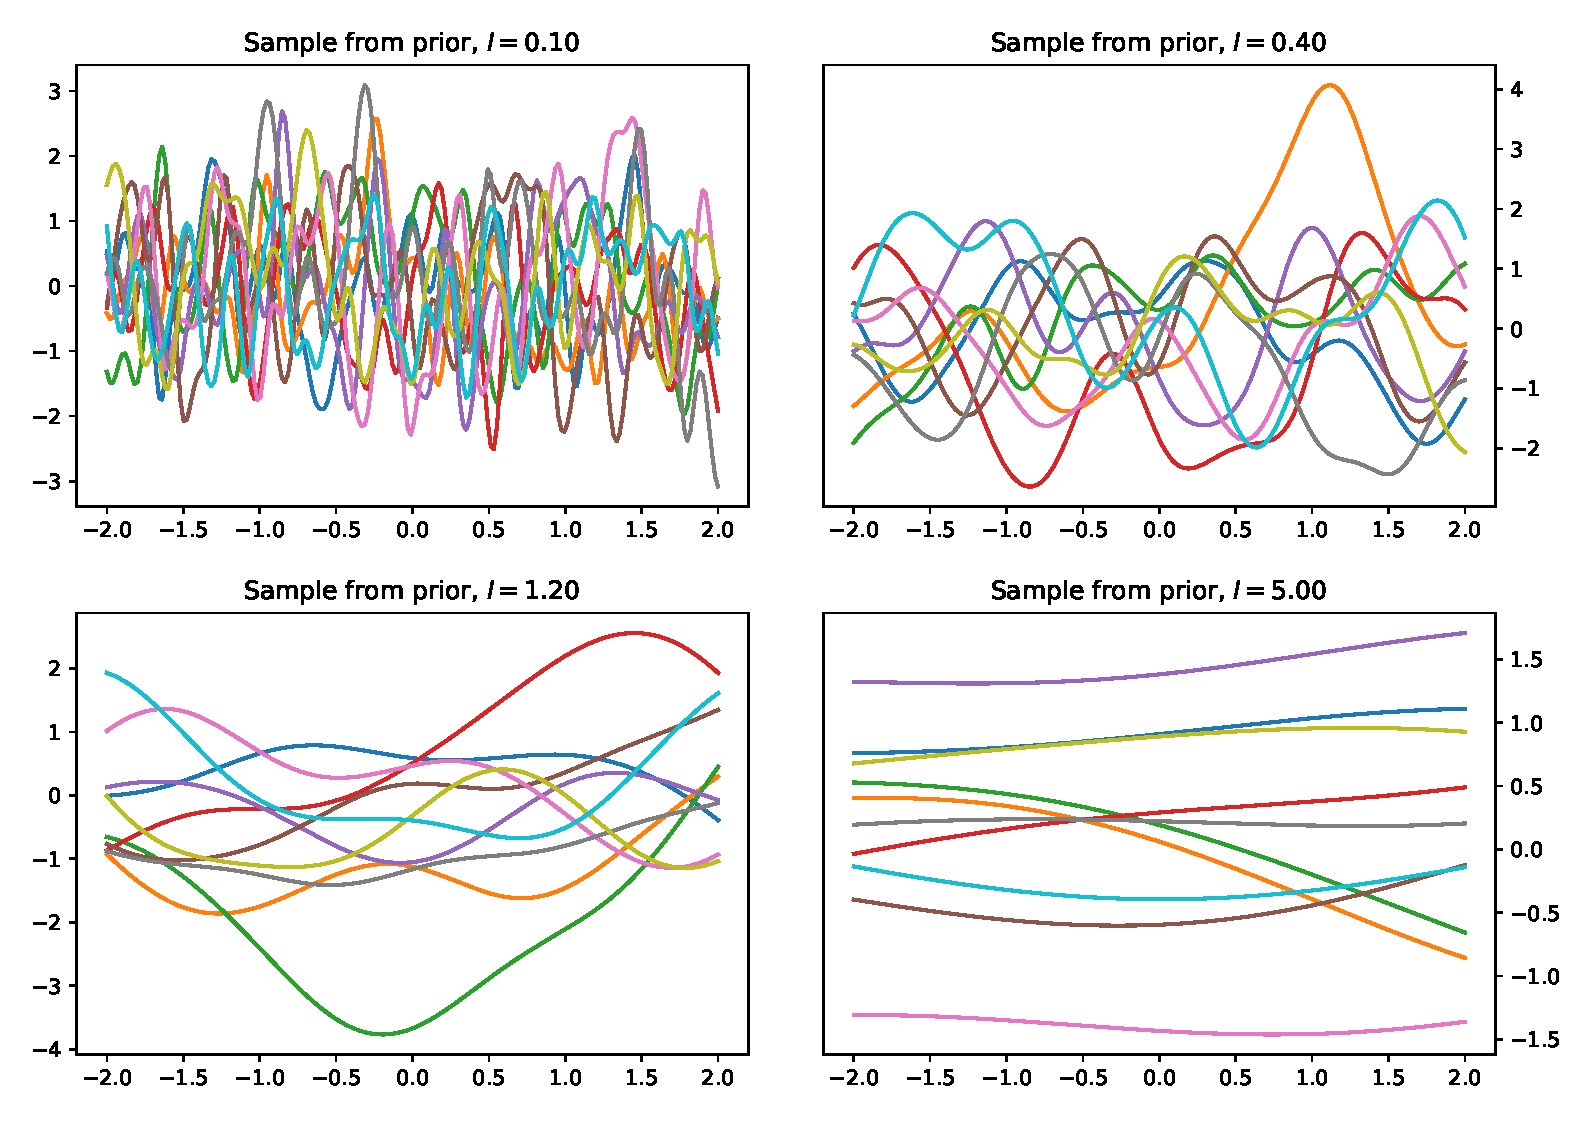
\includegraphics[width=1\textwidth]{GPprior.eps}
	\caption{\label{fig:frog} Samples taken from the squared exponential $\mathcal{GP}$-prior for different length-scales.}
\end{figure}

\noindent We see that using a larger length-scale results in smoother curves, looking at the expression for the kernel,

\begin{equation*}
k(\mathbf{x}_i,\mathbf{x}_j)=\sigma^2\exp\bigg(-\frac{\vert \mathbf{x}_i-\mathbf{x}_j\vert^2}{l^2}\bigg)
\end{equation*} 

\noindent we can conclude that the size of the length-scale indicates how much correlation we expect $f(\mathbf{x}_i)$ and $f(\mathbf{x}_j)$ to have. Larger $l$-values means high correlation (at most equal to $\sigma^2$) so we expect samples to be similar resulting in smoother curves. Small values result in samples tending to what looks like white noise i.e. no correlation between $f_i$'s.

\newpage

\noindent\textbf{Q11}

\noindent\makebox[\linewidth]{\rule{\textwidth}{0.4pt}}
\hfil

\noindent We know that the posterior will also be a $\mathcal{GP}$ with mean $\mathbf{m}_p$ and covariance $\mathbf{k}_p$ (lecture slides) given by

\begin{equation*}
\mathbf{m}_p=k(\mathbf{x}_*,\mathbf{X})K(\mathbf{X,X})^{-1}\mathbf{y},\qquad \mathbf{k}_p = k(\mathbf{x}_*\mathbf{x}_*)-k(\mathbf{x}_*,\mathbf{X})^TK(\mathbf{X,X})^{-1}K(\mathbf{X},\mathbf{x}_*).
\end{equation*} 

\noindent Where the subscript asterisk indicate test inputs. If no data is available, the above expressions reverts to those defined in the prior, meaning they are the same if nothing has been observed. This can also be confirmed by inspection of figure 6, where we clearly see that in regions where no data has been observed the mean goes to zero. We can also compare the bottom graph of the same figure with the bottom left one in figure 5 where the same length scale was used, in regions where we have no data, the posterior is indeed similar to the prior. What can also be observed is that the uncertainty is smaller in regions where we have more data, which is reasonable indeed.

\begin{figure}[H]
	\centering
	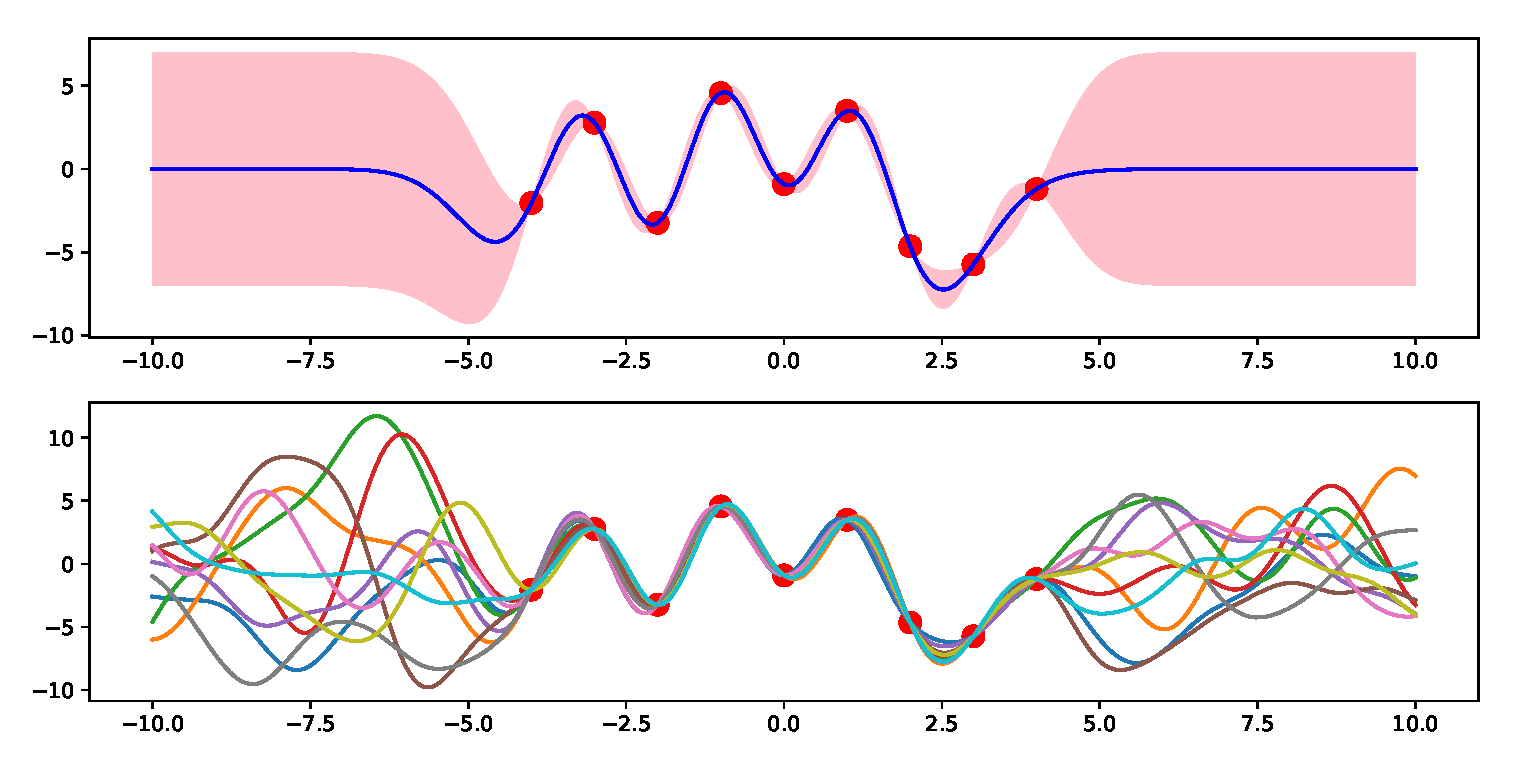
\includegraphics[width=0.7\textwidth]{GPosterior.eps}
	\caption{\label{fig:frog} The top graph show the mean of the posterior with the pink area corresponding the mean plus minus 2 std. The bottom graph show 10 samples taken from the posterior. Red dots correspond to noisy data samples. The length-scale was set to 1.2.}
\end{figure}

\begin{figure}[H]
	\centering
	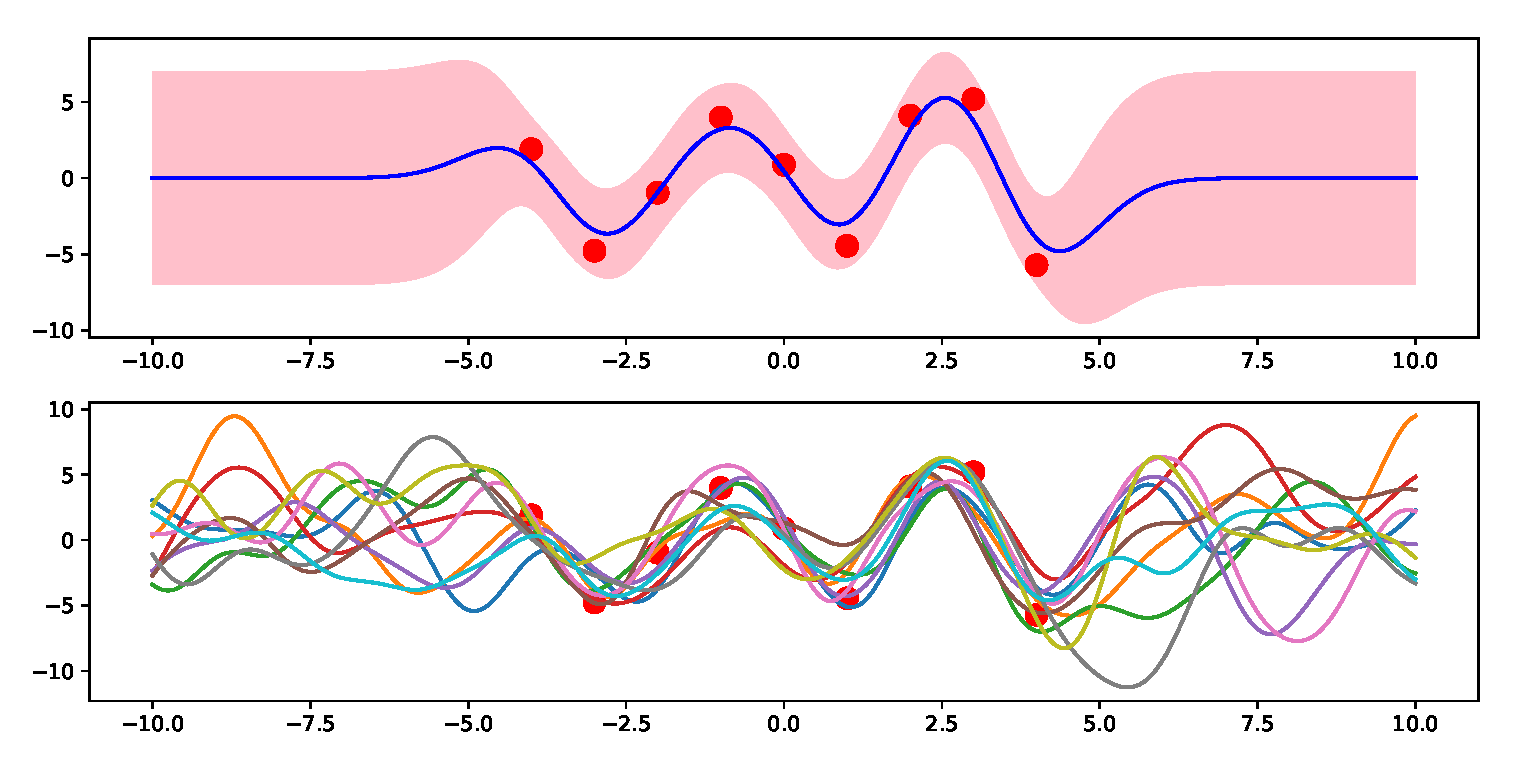
\includegraphics[width=0.7\textwidth]{GNoisePosterior.eps}
	\caption{\label{fig:frog} The top graph show the mean of the posterior with an added diagonal covariance matrix to the squared exponential. The bottom graph show 10 samples taken from the posterior. Red dots correspond to noisy data samples. The length-scale was set to 1.2.}
\end{figure}

\noindent In figure 7 we see the effect of adding a diagonal covariance matrix to the squared exponential, it corresponds to assuming that there is noise in the space of the function realizations leading to posterior samples not necessarily passing through the data points.

\section{The Posterior}

\noindent\textbf{Q12}

\noindent\makebox[\linewidth]{\rule{\textwidth}{0.4pt}}
\hfil

\noindent Using a prior

\begin{equation*}
p(\mathbf{X})=\mathcal{N}(\mathbf{0,I})
\end{equation*} 

\noindent encodes preference for independence between variables, and values for each to be centered around zero with unit variance.
 
\hfil

\noindent\textbf{Q13}

\noindent\makebox[\linewidth]{\rule{\textwidth}{0.4pt}}
\hfil

\noindent We know that the marginal distribution is Gaussian and from the linear relations between $\mathbf{Y}$ and $\mathbf{X}$ together with our prior assumption about $\mathbf{X}$, we can look at the mean and covariance directly using a single data point. ($\epsilon\sim\mathcal{N}(\mathbf{0},\beta^2\mathbf{I})$).

\begin{align*}
\E\big[\mathbf{\mathbf{y}\vert W}\big] =\E\big[\mathbf{Wx}+\epsilon\big]=\mathbf{W}\E\big[\mathbf{x}\big] + \E\big[\epsilon\big] = \mathbf{0},\\
\text{cov}\big[\mathbf{y\vert W,y\vert W}\big]= \E\big[\big(\mathbf{Wx+\epsilon}\big)\big(\mathbf{Wx+\epsilon}\big)^T\big]=\\\E\big[\mathbf{Wxx}^T\mathbf{W}^T\big]+\E\big[\epsilon\epsilon^T\big]=\\ \mathbf{WW}^T+\beta^2\mathbf{I}.
\end{align*}

\noindent This holds for all inputs and outputs, meaning we can generalize and conclude that $p(\mathbf{Y\vert W})=\mathcal{N}(\mathbf{0},\mathbf{WW}^T+\beta^2\mathbf{I})$.

\hfil

\noindent\textbf{Q14}

\noindent\makebox[\linewidth]{\rule{\textwidth}{0.4pt}}
\hfil

\noindent Looking at the three different negative logs for these approaches

\begin{align*}
\mathcal{L}(\mathbf{W})_{ML}=-\ln(p(\mathbf{Y}\vert\mathbf{X},\mathbf{W}))=\ln(Z_{ML})+\frac{1}{2\sigma^2}\tr\bigg[\big(\mathbf{Y}-\mathbf{WX}\big)^T\big(\mathbf{Y}-\mathbf{WX}\big)\bigg],
\end{align*}

\begin{align*}
\mathcal{L}(\mathbf{W})_{MAP}=-\ln\big(p(\mathbf{Y}\vert\mathbf{X},\mathbf{W}&)p(\mathbf{W})\big)=\ln(Z_{MAP}) + \\&+\tr\bigg[\frac{1}{2\sigma^2}\big(\mathbf{Y}-\mathbf{WX}\big)^T\big(\mathbf{Y}-\mathbf{WX}\big)+\frac{1}{2\tau^2}\mathbf{WW}^T\bigg],
\end{align*}

\begin{align*}
\mathcal{L}(\mathbf{W})_{ML_{T2}}=-\ln(p(\mathbf{Y}\vert\mathbf{W}))=\ln(Z_{ML_{T2}}(\mathbf{W}))+\frac{1}{2}\tr\bigg[\mathbf{Y}^T\big(\mathbf{WW}^T+\beta^2\mathbf{I}\big)^{-1}\mathbf{Y}\bigg].
\end{align*}

\noindent We see that the $ML$ treatment is very dependent on the data, thus in order for it to converge we need lots of it and is prone to over-fitting else-wise. $MAP$ includes a prior belief on our model and is thus more of a Bayesian approach, which generalizes better with less data available due to the regularization term that comes with it. A significant difference between the two is that the first will find the mode of the likelihood while the other finds the mode of the posterior, which will be approximately equal as we see more data due to the regularization term becoming less impactful. Type 2 $ML$ averages over all the data i.e. marginalizes it out before we submit to a maximization and uses a prior belief, attributing it to being the most Bayesian treatment. We also note that the distribution wont depend on $\mathbf{X}$, making it sensible to use over the other two.

The last two expressions in Eq. 25 are equal since the denominator in the first does not depend on $\mathbf{W}$, it has been marginalized out.   

\hfil

\noindent\textbf{Q15}

\noindent\makebox[\linewidth]{\rule{\textwidth}{0.4pt}}
\hfil

\noindent Assuming $\mathbf{W}\in\mathbb{R}^{D\times q}$, $\mathbf{Y}\in\mathbb{R}^{D\times n}$, we have

\begin{align*}
\mathcal{L}(\mathbf{W})=\ln(A)+\frac{n}{2}\ln\bigg(\vert\mathbf{\Sigma}\vert\bigg)+\frac{1}{2}\tr\bigg[\mathbf{Y}\mathbf{Y}^T\mathbf{\Sigma}^{-1}\bigg],
\end{align*}

\noindent where $A=(2\pi)^{DN/2}$ and $\mathbf{\Sigma}=\mathbf{WW}^T+\beta^2\mathbf{I}$. To find the gradient with respect to $\mathbf{W}$ we make use of the relations

\begin{align*}
\partial\big(\tr\big(\mathbf{X}\big)\big)&=\tr\big(\partial\mathbf{X}\big),\\
\partial\big(ln\big(\det\big(\mathbf{X}\big)\big)\big)&=\tr\big(\mathbf{X}^{-1}\partial\mathbf{X}\big),\\
\partial\big(\mathbf{X}^{-1}\big)&=-\mathbf{X}^{-1}\big(\partial\mathbf{X}\big)\mathbf{X}^{-1}.
\end{align*}

\noindent We get

\begin{align*}
\frac{\partial\mathcal{L}}{\partial\mathbf{W}}&=\frac{1}{2}\tr\bigg[n\mathbf{\Sigma}^{-1}\frac{\partial\mathbf{\Sigma}}{\partial\mathbf{W}}+\mathbf{Y}\mathbf{Y}^T\frac{\partial\mathbf{\Sigma}^{-1}}{\partial\mathbf{W}}\bigg] \\&= \frac{1}{2}\tr\bigg[n\mathbf{\Sigma}^{-1}\frac{\partial\mathbf{\big(\mathbf{WW}^T\big)}}{\partial\mathbf{W}}-\mathbf{Y}\mathbf{Y}^T\mathbf{\Sigma}^{-1}\frac{\partial\big(\mathbf{WW}^T\big)}{\partial\mathbf{W}}\mathbf{\Sigma}^{-1}\bigg]\\&=\frac{1}{2}\tr\bigg[\underbrace{\bigg(n\mathbf{\Sigma}^{-1}-\mathbf{\Sigma}^{-1}\mathbf{Y}\mathbf{Y}^T\mathbf{\Sigma}^{-1}\bigg)}_{=\mathbf{\Lambda}}\frac{\partial\big(\mathbf{WW}^T\big)}{\partial\mathbf{W}}\bigg].
\end{align*}

\noindent The gradient can then be defined by the element-wise derivative with help of the Singleentry Matrix $\mathbf{J}^{ij}$ and Petersen and Pedersen 2006 eq. 80

\begin{equation*}
\frac{\partial \mathcal{L}}{\partial W_{i,j}}=\frac{1}{2}\tr\bigg[\mathbf{\Lambda}\frac{\partial\big(\mathbf{WW}^T\big)}{\partial W_{i,j}}\bigg],\quad\text{where}\quad\frac{\partial\big(\mathbf{WW}^T\big)}{\partial W_{i,j}}=\mathbf{J}^{ij}\mathbf{W}^T+\mathbf{W}\big(\mathbf{J}^{ij}\big)^T.
\end{equation*} 


\newpage
\noindent\textbf{Q16}

\noindent\makebox[\linewidth]{\rule{\textwidth}{0.4pt}}
\hfil

\noindent In the following figure we see both the original function and the learned one for two instantiations.  

\begin{figure*}[h!]
	\centering
	\begin{subfigure}[t]{0.5\textwidth}
		\centering
		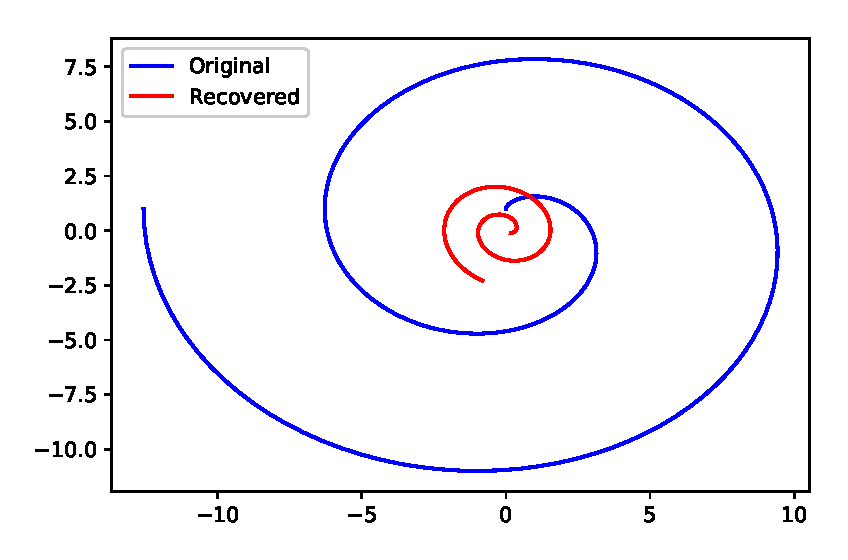
\includegraphics[height=1.5in]{representation.eps}
	\end{subfigure}%
	~ 
	\begin{subfigure}[t]{0.5\textwidth}
		\centering
		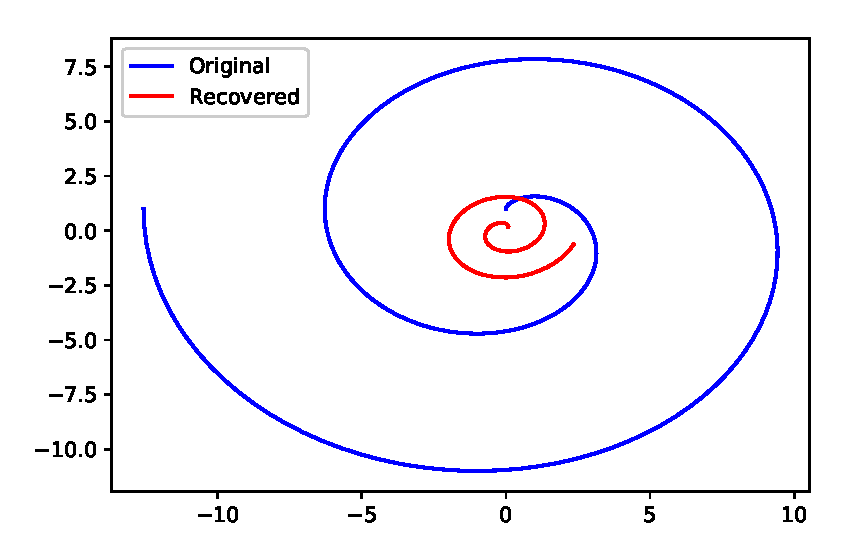
\includegraphics[height=1.5in]{representation2.eps}
	\end{subfigure}
\caption{Result of two instantiations related to Q16.}
\end{figure*}

\noindent It is clear that certain properties were recovered from the original, but some were lost as-well. In particular, the two recovered mappings were similar in that they 'spiraled' in the same direction but differed in orientation by some phase. The scale of the recovered mappings underestimated the original consistently during many instantiations. The origin of the scale difference is hard to pin-point (it might have to do with the mapping not being one-to-one), but the phase shift occurrence can be explained from the redundancy in the parameterization corresponding to rotations of the latent space coordinates, this can be seen by considering a matrix $\tilde{\mathbf{W}}=\mathbf{WR}$ where $\mathbf{R}$ is an orthogonal matrix (or rotation matrix). Looking at the marginal distribution $\mathcal{N}(\mathbf{0},\mathbf{\tilde{\mathbf{W}}}\tilde{\mathbf{W}}^T+\beta\mathbf{I})=\mathcal{N}(\mathbf{0},\mathbf{\mathbf{W}}\mathbf{W}^T+\beta\mathbf{I})$, meaning that there's a lot of different $\tilde{\mathbf{W}}$ that give rise to the same distribution. 

\hfil

\section{The Evidence $p(\mathcal{D})$}

\noindent\textbf{Q17}

\noindent\makebox[\linewidth]{\rule{\textwidth}{0.4pt}}
\hfil

\noindent As is discussed in the paper (Murray and Z. Ghahramani), one could argue that model complexity is tied to the number of parameters of the model. This would imply that $M_0$ is as simple as can be given it has zero parameters. It's bad in that it does not take any data into consideration except its cardinality, and it's not very flexible due to being constant over all of $\mathcal{D}$ making it very restricted in its ability to assign much probability mass to simple sets of data. It does however have the advantage of having the largest evidence over all the data sets since it spreads its probability mass uniformly, and also; it's computationally efficient since we don't have to estimate any parameter.

\newpage

\noindent\textbf{Q18}

\noindent\makebox[\linewidth]{\rule{\textwidth}{0.4pt}}
\hfil

\noindent In $M_1$, a parameter $\theta_1^1$ is introduced. Looking at its structure; $M_1$ takes only the first argument of each $\mathbf{x}^i$ into account, thus limiting it to only being able to generate linear decision boundaries that are functions of said argument that go through the origin. Since $M_1$ is specialized at fitting to data that suits its boundaries, it will concentrate its probability mass to those data sets, meaning that it will have lower evidence elsewhere, thus $M_0$ might be a better fit for some other data sets as it spreads its probability mass uniformly.

\hfil

\noindent\textbf{Q19}

\noindent\makebox[\linewidth]{\rule{\textwidth}{0.4pt}}
\hfil

\noindent First of all we note that each $M_i$ where $i>0$ can be reduced to $M_0$ by setting their respective $\boldsymbol{\theta}_i$ to zero. Thus we can look at the models as being more flexible with increasing $i$ in a rather linear fashion.

$M_2$ gains one more degree of freedom compared to $M_1$, in that it also looks at the second argument of $\mathbf{x}^i$, this allows for decision boundaries that depend on both but still have to travel through the origin. Taking this even further, $M_3$ has the ability to translate its decision boundaries from the origin due to the new bias term $\theta_3^3$, making it capable to capture a different kind of structure in the data compared to the less flexible models.  

What can be said about increasing the number of parameters for model 1 through 3 is that the higher you go; the more the probability mass will be spread over the different possible data sets. Meaning that if a simple model explains observed data well, then, even if a more complex model can revert to the former, it is constrained from being able to have as high evidence as the simpler model due to its probability mass being spread wider.

\hfil

\noindent\textbf{Q20}

\noindent\makebox[\linewidth]{\rule{\textwidth}{0.4pt}}
\hfil

\noindent Due to using a distribution perspective i.e. being 'Bayesian' and thinking that the parameters $\boldsymbol{\theta}_i$ should be represented by a belief, there are infinitely many versions of model $M_i$ to choose from. So in order to present evidence of how representative a model is for some data, (given that we are uncertain of its parameters) we use marginalization in order to remove this dependence of how we need to present an explicit $\boldsymbol{\theta}_i$ to evaluate a model. The integration can be viewed then as a weighted average over all different parameters.

\hfil

\noindent\textbf{Q21}

\noindent\makebox[\linewidth]{\rule{\textwidth}{0.4pt}}
\hfil

\noindent 

\end{document}